\section{Implementáció}

\subsection{Fejlesztő környezet}

Mind a kliens, mind a szerver oldal implementálása Java nyelven történik. A kliens oldal az Ericsson Service Development Studio (SDS) 4.1 fejlesztőeszköz segítségével valósult meg. Az SDS az Ericsson honlapján 2010 végéig egy szabadon hozzáférhető fejlesztő környezet volt, jelenleg az alkalmazás támogatása megszűnt, így az le sem tölthető\footnote{Az eszközt, valamint a dokumentációt még korábban, az egyetemi önálló labor keretein belül szereztem be.}. A fejlesztőeszköz képes emulálni az IMS hálózat főbb funkcionális egységeit, így lehetőséget teremt IMS hálózatra szánt alkalmazások fejlesztésére, valamint azok tesztelésére. Az SDS a nyílt forráskódú Eclipse fejlesztői környezetre épül, így az egész rendszer bármilyen, Microsoft Windows XP operációs rendszert futtató PC-n használható. Szabványosított API-kat használhatunk kliens és szerveroldali programozáshoz, valamint a kommunikációs folyamatok, szolgáltatások megvalósításához egyaránt. A fejlesztői keretrendszerbe beépített tesztelési egységek lehetőséget nyújtanak végpontól végpontig tartó tesztelésre. Az SDS tartalmaz előre elkészített funkciókat is, amelyeket a fejlesztők felhasználhatnak az új szolgálatások elkészítése során. Ilyen funkció például a jelenlét, csoport és adatkezelés (Presence, Group and Data Management), amely funkciót az általam fejlesztett csoportos üzenetküldő szolgáltatásban is használok.

\subsubsection{Az SDS IMS maghálózat támogatása}

A fejlesztői PC-n kialakított, SDS által nyújtott IMS emulációs környezet felépítése \aref{fig:sds_env}.~ábrán  látható. Mint ahogy az ábrán is látható, az SDS IMS környezeti emulátorokat (CSCF, DNS, HSS, IMS Proxy), valamint az elkészült szerveroldali alkalmazások futtatásához SIP alkalmazás szervert tartalmaz. Lehetőségünk van saját SIP alkalmazás szervert üzembe állítani, majd az SDS-t úgy konfigurálni, hogy az általunk kívánt alkalmazás szervert használja\footnote{A szerveroldali szolgáltatás futtatásához a BEA Weblogic SIP Server 3.1-es verzióját használtam. \cite{bea_weblogic}}. 

\begin{figure}[htbp]
\center
\resizebox{14cm}{!}{
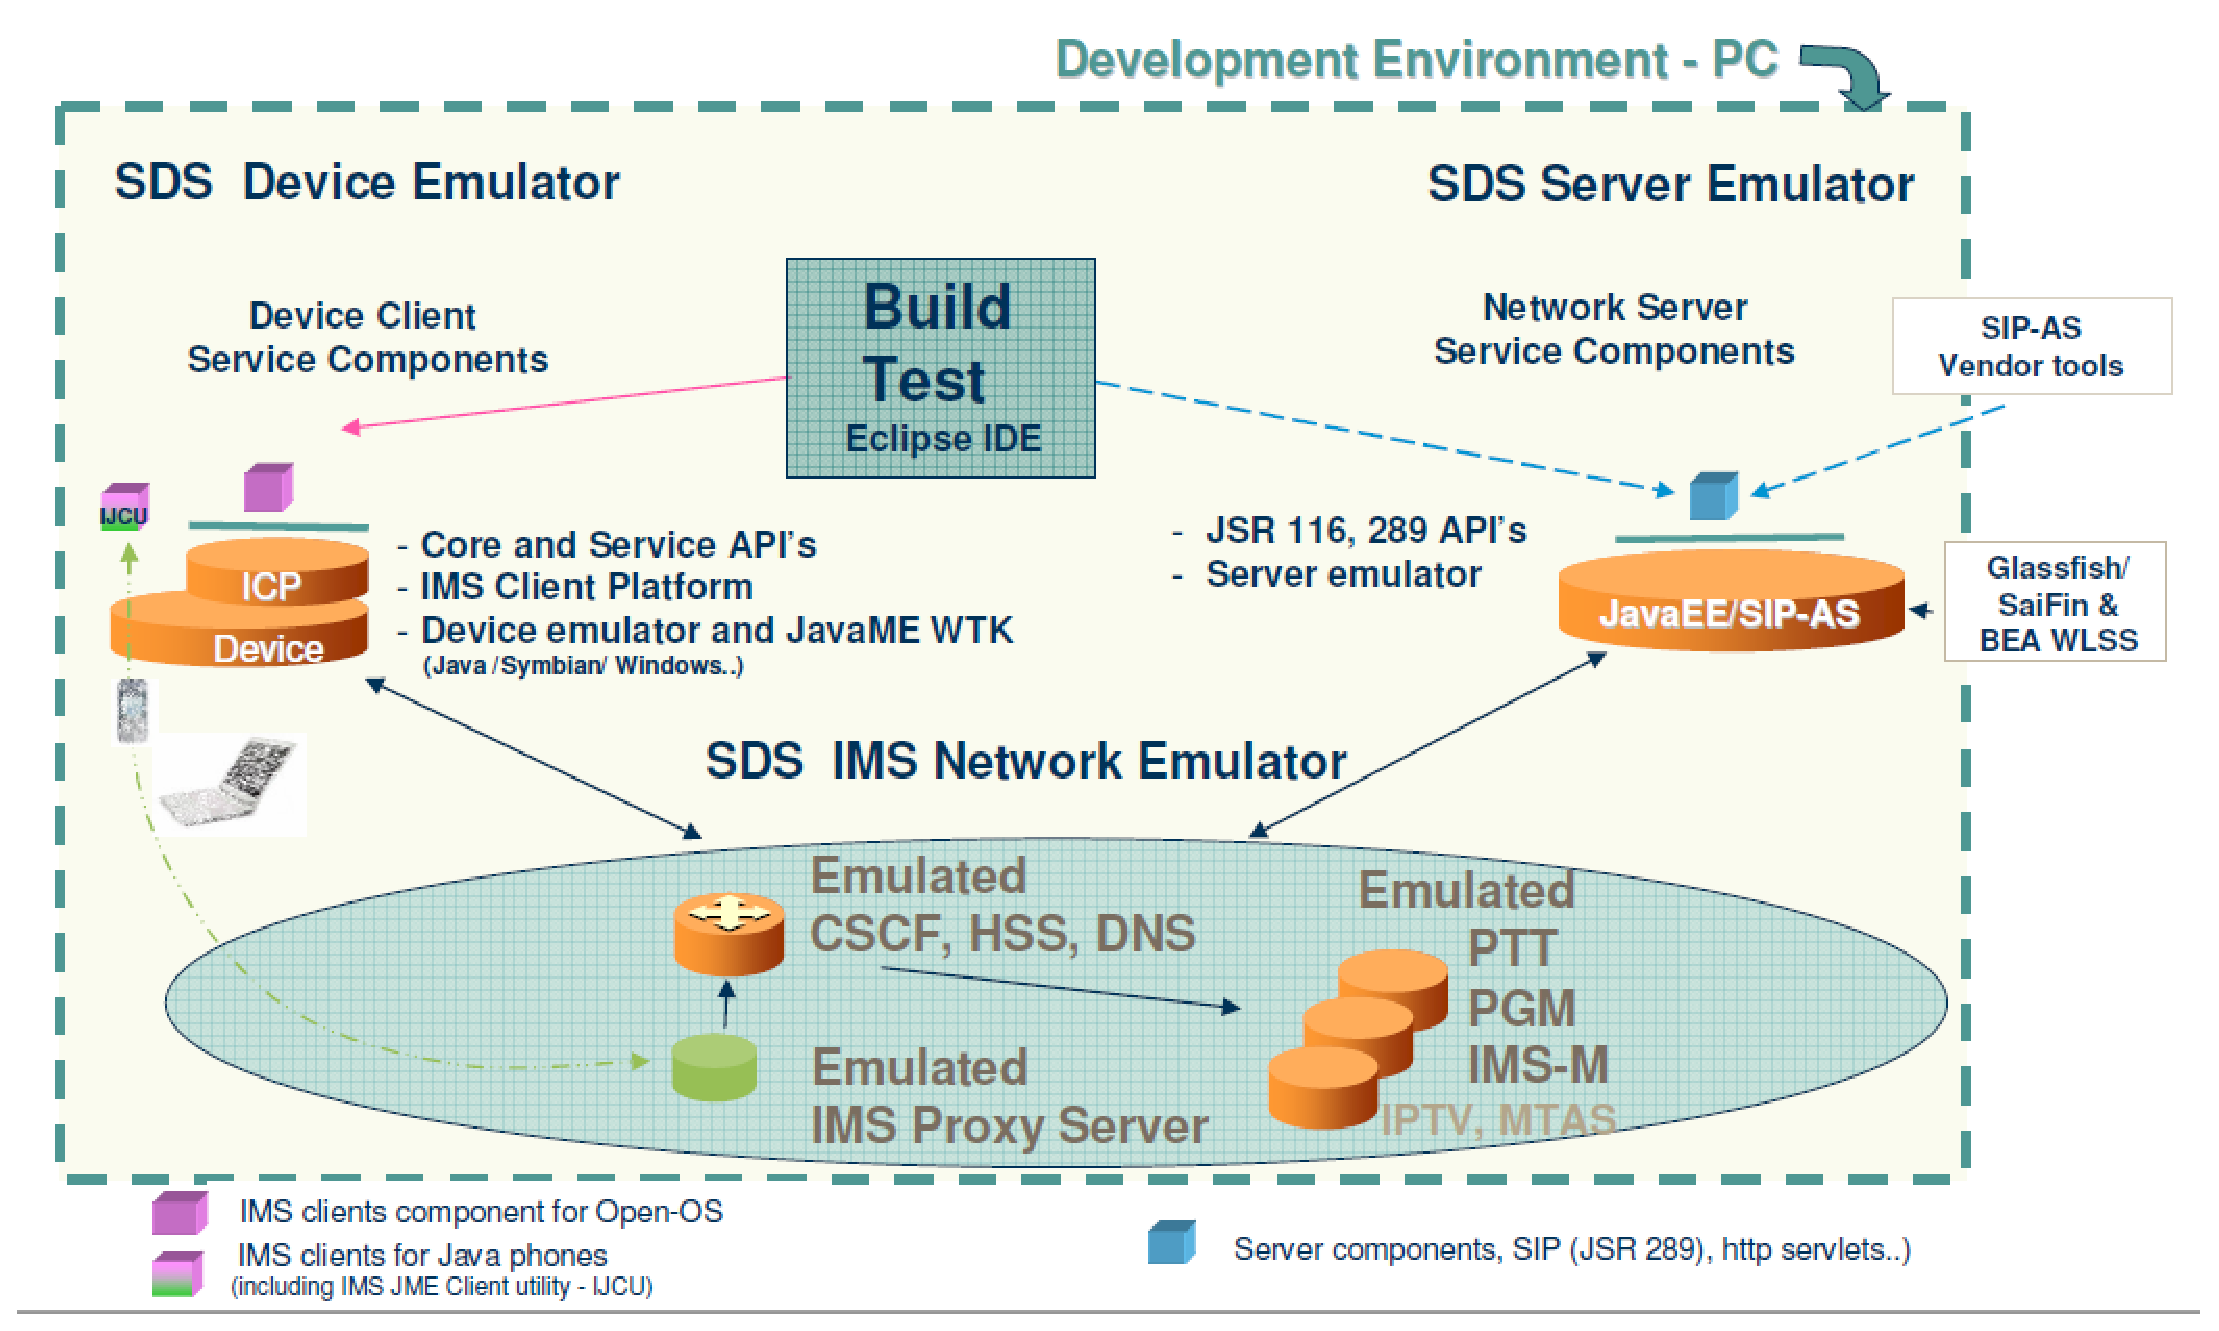
\includegraphics{img/sds-overview.eps}}
\caption{A fejlesztői PC-n kialakított emulációs környezet felépítése~\cite{sds_tech_desc}}
\label{fig:sds_env}
\end{figure}

Az IMS eszközök legfontosabb beállításait az Eclipse IDE Provisioning nézetében tekinthetjük meg, illetve módosíthatjuk. Itt található a registrar, amely az aktuálisan a CSCF-hez beregisztrált felhasználókat táblázatos formában jeleníti meg. A HSS fül alatt hozhatunk létre felhasználókhoz rendelhető profilokat. Itt hozhatunk létre IFC-ket (Initial Filter Criteria), valamint SPT-ket (Service Point Trigger). Az SPT egy összetett logikai kifejezés, amely a SIP üzenetek bizonyos tulajdonságaira létrehozható logikai állítás. Ilyen logikai állítás lehet a SIP üzenet típusára tett megkötés, vagy a SIP üzenet fejlécére vonatkozó állítás, valamint a request URI-ra tett állítás. Az SPT-t összefoghatóak egyetlen IFC-be, amely tulajdonképpen belépési pont az alkalmazásokhoz. Ilyen módon egyszerűen, logikai állítások halmazával meghatározható, hogy bizonyos feltételek teljesülése esetén mely alkalmazások legyenek értesítve. A létrehozható profilok lényegében IFC-k halmaza. Ezáltal egy felhasználóhoz rendelt profil meghatározza, hogy a felhasználó melyik szolgáltatások használatára jogosult, és melyikre nem. 

\subsubsection{Az SDS kliens oldali készülékek támogatása}

Az SDS kliens oldali fejlesztéshez is nyújt eszközt, amely az IMS Client Framework (ICF) nevet kapta. Az ICF-nek két fő része van. 

Az egyik az IMS Client Platform (ICP), amely Windows vagy Symbian platformra nyújt olyan keretrendszert, amely tartalmazza az alapvető IMS szolgáltatásokat, mint például a SIP session menedzsment, vagy a már \ref{sec:group_messaging}.~fejezetben említett PGM szolgáltatás.

Az ICF keretrendszer másik része az IMS Java Client Utility (IJCU). Az IJCU olyan J2ME-t támogató telefonokhoz szolgáltat API-t, amelyek nem támogatják a SIP protokollt. Az ilyen eszközök előtt az IJCU transparensen elrejti a SIP protokollt, és HTTP üzenetekbe ágyazva küld és fogad SIP csomagokat.

\subsection{Az MSRP protokoll megvalósítása}
\label{sec:msrp_implementacio}

Az Interneten nem találtam Java nyelven íródott, az MSRP funkcióit megvalósító, használható fejlesztői könyvtárat, ezért a fejlesztés során szükségesnek tartottam az MSRP alapfunkciókat ellátó osztályok implementálását is. Itt jegyezném meg, hogy az általam létrehozott MSRP implementáció nem valósítja meg \acite{rfc4975}.~irodalomban leírt MSRP RFC szabvály minden funkcióját, csak az MSRP kapcsolaton való üzenetküldéshez szükséges alapfunkciókat. Az általam megvalósított részek követik az MSRP protokoll szabályait\cite{rfc4975}. Ebben a részben a multimédia tartalom hálózaton történő átviteléért felelős MSRP funkciókat megvalósító osztályokat mutatom be.  \Aref{tab:msrp_classes}.~táblázatban az említett osztályokat sorolom fel, kiegészítve a felelősségük, funkciójuk rövid leírásával. Az osztályok részletes leírása a fejezet későbbi szakaszában kerül kifejtésre.

\begin{table}[htb]
\center
\begin{tabular}{|l | p{9cm} |}
\hline
{\bf Az osztály neve} & {\bf Az osztály felelőssége}\\
\hline
\hline
Message & Az MSRP üzenetek kötelező paramétereit tartalmazó osztály\\ \hline
Request & Az MSRP kéréseket reprezentáló osztály\\ \hline
Response & Az MSRP válasz típusú üzenetek adatainak tárolása\\ \hline
CompleteMSRPMessage & A teljes üzenetet reprezentáló osztály, amit az MSRP kapcsolaton kívánunk elküldeni\\ \hline
MSRPStack & Az MSRP funkciók elérése MSRP-n kívüli osztályokból\\ \hline
Connections & Az MSRP kapcsolatokat kiszolgáló TCP kapcsolatok tárolása, kezelése\\ \hline
ReceiverConnection & A TCP kapcsolat, amelyen MSRP csomagokat bájtfolyam formájában fogadunk, feldolgozunk\\ \hline
SenderConnection & Különálló kapcsolat az MSRP csomagok küldésére. Minden MSRP kapcsolathoz tartozik egy példánya\\ \hline
Session & Az MSRP kapcsolatot reprezentáló osztály\\ \hline
TransactionManager & Az MSRP csomagok tranzakcionált küldéséért felelős, valamint nyugtázási funkciókat lát el\\ \hline
OutgoingMessageProcessor & Az MSRP kapcsolaton küldött üzenet MSRP kérésekbe való ,,darabolása'', MSRP kérések generálása\\ \hline
IncomingMessageProcessor & Az MSRP kapcsolaton érkező üzenetek feldolgozása, továbbítása a tranzakció menedzser felé\\ \hline
MSRPEvent & Az MSRP kapcsolatban bekövetkezett esemény\\ \hline
MSRPListener & Interfész, az MSRP eseményről való értesítő funkciót lát el\\ \hline
MSRPUtil & Az MSRP üzenet példányok előállítása, üzenet konverziós funkciók\\ \hline
SessionDescription & Az MSRP kapcsolat SDP leíró információit tartalmazó osztály\\ \hline
\hline
\end{tabular}
\caption{Az MSRP funkciókat megvalósító osztályok}
\label{tab:msrp_classes}
\end{table}

\subsubsection*{A Message osztály}
\label{sec:msrp_message}

\begin{wrapfigure}{r}{0.45\textwidth}
  \vspace{-15pt}
  \begin{center}
    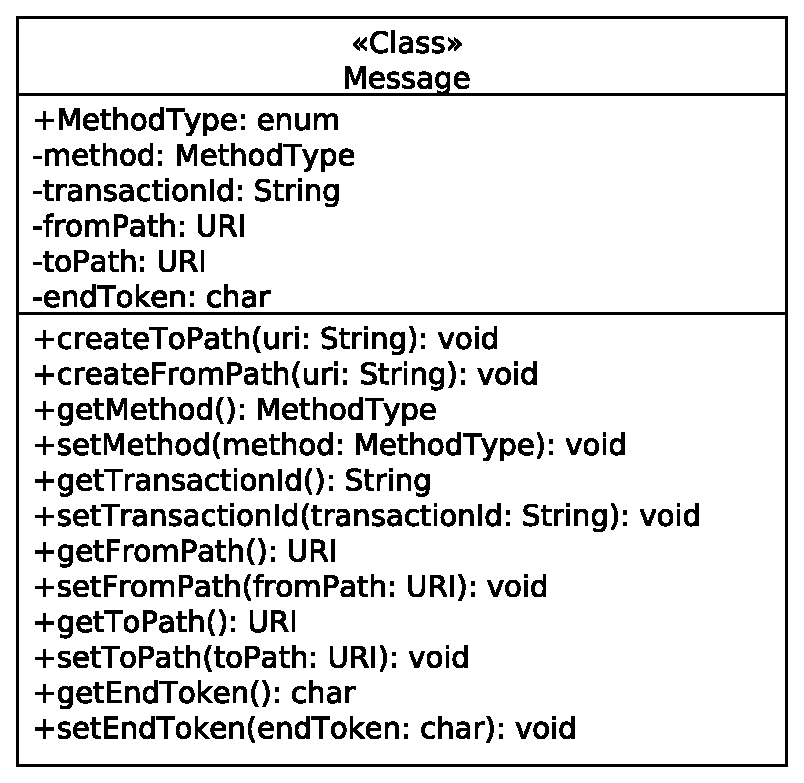
\includegraphics[width=0.43\textwidth]{img/class_diagrams/Message.eps}
  \end{center}
  \vspace{-15pt}
  \captionsetup{font=scriptsize}
  \caption{A Message osztálydiagramja}
   \label{fig:class_message}
  \vspace{-10pt}
\end{wrapfigure}
A \code{Message} osztály (\ref{fig:class_message}.~ábra) tartalmazza azokat adatokat, amelyeket minden MSRP csomagban el kell helyezni. Az üzenet típusa -- esetemben kérés (SEND) vagy nyugta (200 OK) -- a \code{method} változóban tárolódik. Mivel az MSRP csomagok átvitele tranzakcióban zajlik (küldés -- nyugtázás), így minden csomagnak egyedi tranzakció azonosítója kell, hogy legyen (\code{transactionId}). Az MSRP üzenetek fejlécében el kell helyezni az MSRP session lokális és távoli azonosítóját is (\code{toPath}, \code{fromPath}). Utóbbi két változó értéke a \code{Session} osztály \code{remoteURI} és \code{localURI} változóinak értéke (lásd. \ref{sec:msrp_session}.~pont) kiegészítve az átviteli protokollal (amely minden esetben TCP). Végül eltárolásra kerül az MSRP csomag végét lezáró karakter (\$, +, vagy  \# karakter). A paraméterek módosítására, illetve lekérdezésére metódusok állnak rendelkezésre.

\subsubsection*{A Request osztály}
\label{sec:msrp_request}

\begin{wrapfigure}{r}{0.45\textwidth}
  \vspace{-15pt}
  \begin{center}
    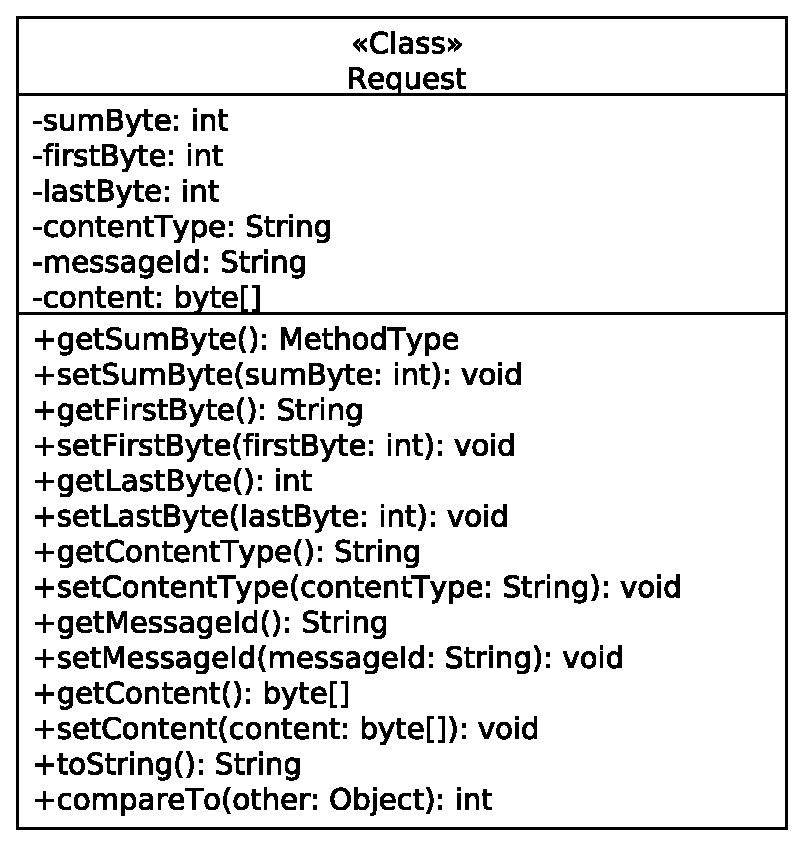
\includegraphics[width=0.43\textwidth]{img/class_diagrams/Request.eps}
  \end{center}
  \vspace{-15pt}
  \captionsetup{font=scriptsize}
  \caption{A Request osztálydiagramja}
   \label{fig:class_request}
  \vspace{-10pt}
\end{wrapfigure}
Az osztály \aref{sec:msrp_message}.~pontban kifejtett \code{Message} osztály leszármazottja. A \code{Request} osztály reprezentálja az MSRP kapcsolatokon küldött MSRP kéréseket. Az osztály a \code{Message} osztályhoz képest \aref{fig:class_request}.~ábrán látható változókkal, metódusokkal bővül. A \code{sumByte} a kérésben átvitelre kerülő teljes MSRP üzenet bájtokban számolt méretét tárolja. Egy teljes MSRP üzenet több kérésben kerül átvitelre, a \code{firstByte} és \code{lastByte} változók a teljes üzenethez képest az aktuális kérésben átvitelre kerülő első és utolsó bájt sorszámát tárolják. A teljes MSRP üzenet azonosítója a \code{messageId} változóba kerül, tehát ugyanazon üzenet más-más darabját ,,hordozó'' MSRP kéréseknek ugyanaz a \code{messageId} értéke kell, hogy legyen. A kérés törzsében átvitt adat típusát a \code{contentType} mező, míg a tényleges tartalmat a \code{content} bájttömb tárolja. 

\subsubsection*{A Response osztály}
\label{sec:msrp_response}

\begin{wrapfigure}{r}{0.45\textwidth}
  \vspace{-15pt}
  \begin{center}
    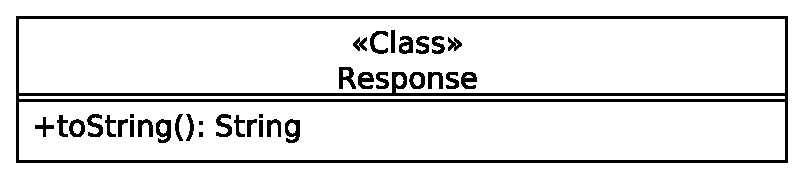
\includegraphics[width=0.43\textwidth]{img/class_diagrams/Response.eps}
  \end{center}
  \vspace{-15pt}
  \captionsetup{font=scriptsize}
  \caption{A Response osztálydiagramja}
   \label{fig:class_response}
  \vspace{-10pt}
\end{wrapfigure}
A \code{Response} osztály (\ref{fig:class_response}.~ábra) szintén az \code{Message} osztály leszármazottja, így minden paraméterrel és metódussal rendelkezik, ami a \code{Message} osztályban szerepel. A \code{Message} osztályhoz képest annyiban nyújt többet, hogy felüldefiniálja az osztály \code{toString()} metódusát.

\subsubsection*{A CompleteMSRPMessage osztály}
\label{sec:msrp_completmsrpemessage}

\begin{wrapfigure}{r}{0.45\textwidth}
  \vspace{-15pt}
  \begin{center}
    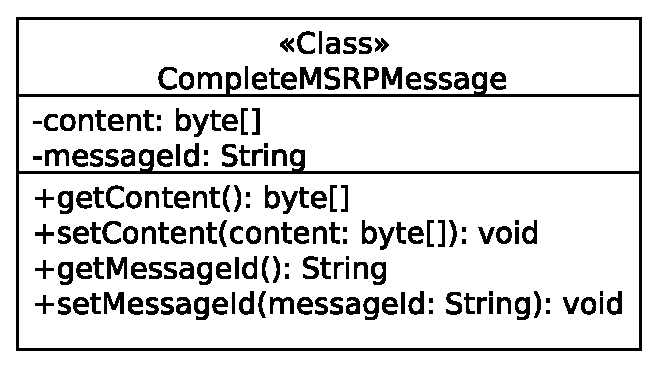
\includegraphics[width=0.43\textwidth]{img/class_diagrams/CompleteMSRPMessage.eps}
  \end{center}
  \vspace{-15pt}
  \captionsetup{font=scriptsize}
  \caption{A CompleteMSRPMessage osztálydiagramja}
   \label{fig:class_completmsrpemessage}
  \vspace{-10pt}
\end{wrapfigure}
A \code{CompleteMessage} osztály osztálydiagramja \aref{fig:class_completmsrpemessage}.~ábrán látható. Az osztály tárolja az MSRP kapcsolaton átküldendő üzenet teljes tartalmát (\code{content}), illetve az üzenet egyedi azonosítóját (\code{messageId}). Az MSRP átvitel során ennek az üzenetnek a tartalmából fognak generálódni \aref{sec:msrp_request}.~pontban tárgyalt MSRP kérés üzenetek. A változók értékeinek lekérdezésére, illetve módosítására metódusok állnak rendelkezésre.

\subsubsection*{Az MSRPStack osztály}
\label{sec:msrp_stack}

\begin{wrapfigure}{r}{0.45\textwidth}
  \vspace{-15pt}
  \begin{center}
    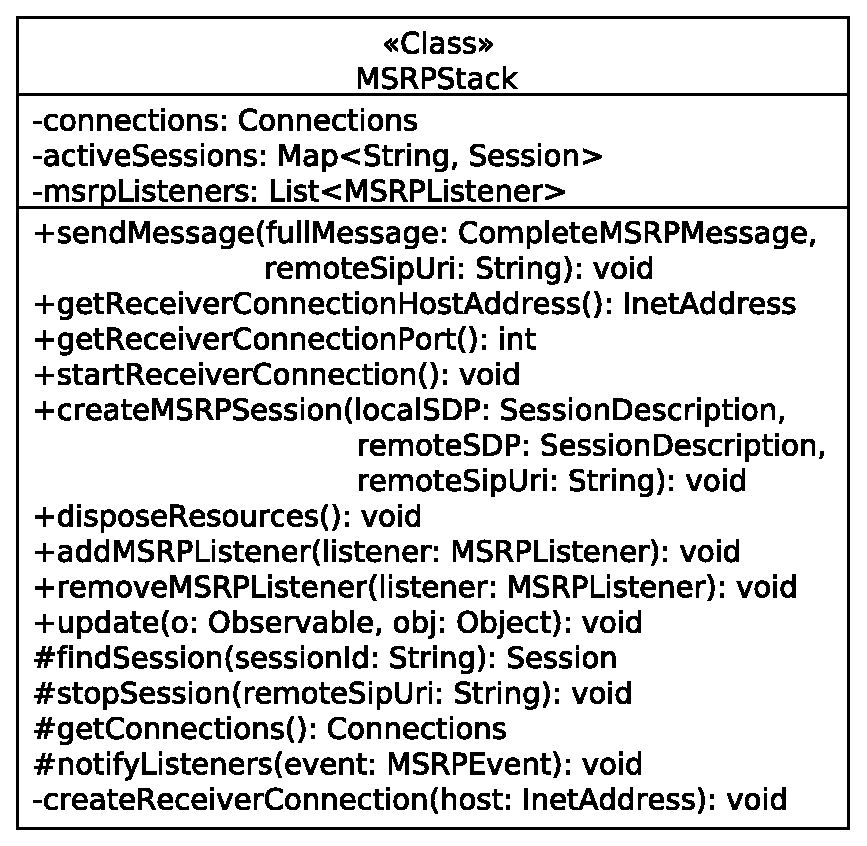
\includegraphics[width=0.43\textwidth]{img/class_diagrams/MSRPStack.eps}
  \end{center}
  \vspace{-15pt}
  \captionsetup{font=scriptsize}
  \caption{Az MSRPStack osztálydiagramja}
  \label{fig:class_msrp_stack}
  \vspace{-10pt}
\end{wrapfigure}
Az \code{MSRPStack} osztály (\ref{fig:class_msrp_stack}.~ábra) feladata az MSRP funkciók nyújtása az alkalmazás számára. Az osztály privát változói között szerepel az MSRP kapcsolatokat kiszolgáló TCP kapcsolatokat kezelő osztály (\code{connections}), az aktív MSRP kapcsolatokat tartalmazó map (\code{activeSessions}), valamint az MSRP eseményekre feliratkozott osztályok listája (\code{msrpListeners}). Az \code{activeSessions} map a távoli fél egyedi SIP URI-ját használja, mint kulcs attribútum. Az osztály segítségével egy távoli fél felé létrehozhatunk új MSRP kapcsolatot (\code{createMSRPSession}). Lekérdezhetünk annak lokális TCP kapcsolatnak az adatait, amelyen keresztül olvashatjuk az aktív MSRP kapcsolatonon beérkező üzeneteket (\code{getReceiverConnectionHostAddress}, \code{getReceiverConnectionPort}). Ha egy meglévő MSRP kapcsolaton üzenetet kívánunk küldeni, akkor ezt a \code{sendMessage} publikus metódus meghívásával tehetjük meg. Az MSRP kapcsolatokat a távoli fél SIP URI-jával azonosítjuk. Egy külső osztály az MSRP eseményekre feliratkozni az \code{addMSRPListener} metódussal, míg az eseményekről leiratkozni a \code{removeMSRPListener} metódus meghívásával tud. A védett (\code{protected}) metódusokat csak az MSRP-t megvalósító osztályok használják.

\subsubsection*{A Connections osztály}
\label{sec:msrp_connections}

\begin{wrapfigure}{r}{0.45\textwidth}
  \vspace{-15pt}
  \begin{center}
    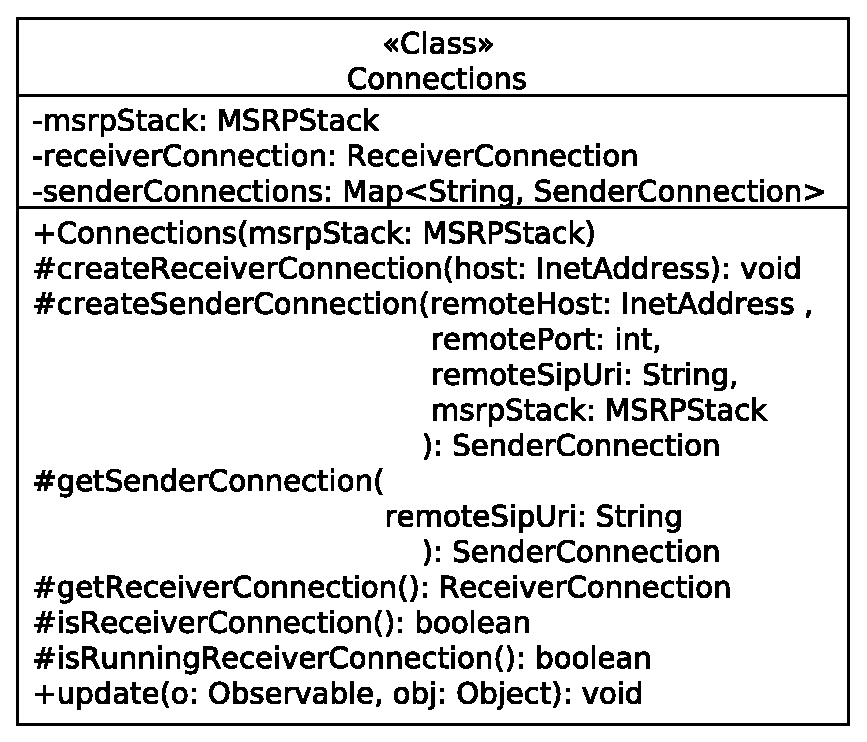
\includegraphics[width=0.43\textwidth]{img/class_diagrams/Connections.eps}
  \end{center}
  \vspace{-15pt}
  \captionsetup{font=scriptsize}
  \caption{A Connections osztálydiagramja}
   \label{fig:class_connections}
  \vspace{-10pt}
\end{wrapfigure}
A \code{Connections} osztály felépítése \aref{fig:class_connections}.~ábrán látható. Az osztály felelős az MSRP kapcsolatokat kiszolgáló, a tényleges adatátvitelért felelős TCP kapcsolatok menedzseléséért. Az osztály metódusaival létrehozhatjuk az MSRP kapcsolatokon beérkező csomagok olvasását megvalósító TCP kapcsolatot (\code{createReceiverConnection}), valamint az MSRP kapcsolatokon küldött adatok átviteléért felelős TCP kapcsolatokat (\code{createSenderConnection}). Mivel az MSRP kapcsolatokon beérkező üzenetek olvasására elegendő egyetlen TCP kapcsolat, így abból csak egy van. Mivel az MSRP csomagok fejléce tartalmazza az MSRP kapcsolat azonosítóját (path attribútum), így a beérkező csomagokról egyértelműen el tudjuk dönteni, hogy azok melyik MSRP kapcsolathoz tartoznak, így a csomagok továbbíthatók a helyes MSRP kapcsolathoz. A távoli félnek küldött MSRP csomagok átvitelét megvalósító TCP kapcsolatokból ellenben többre van szükség, mivel minden távoli félhez külön TCP kapcsolatot kell létrehozni. A küldő kapcsolatokat a \code{senderConnections} mapben tároljuk el. A map kulcsa a távoli fél SIP URI-ja. Az osztály implementálja az \code{Observer} interfészt, ami arra használatos, hogy a TCP kapcsolatok leállításáról értesüljön a \code{Connections} osztályt.

\subsubsection*{A ReceiverConnection osztály}
\label{sec:msrp_receiverconnection}

\begin{wrapfigure}{r}{0.45\textwidth}
  \vspace{-15pt}
  \begin{center}
    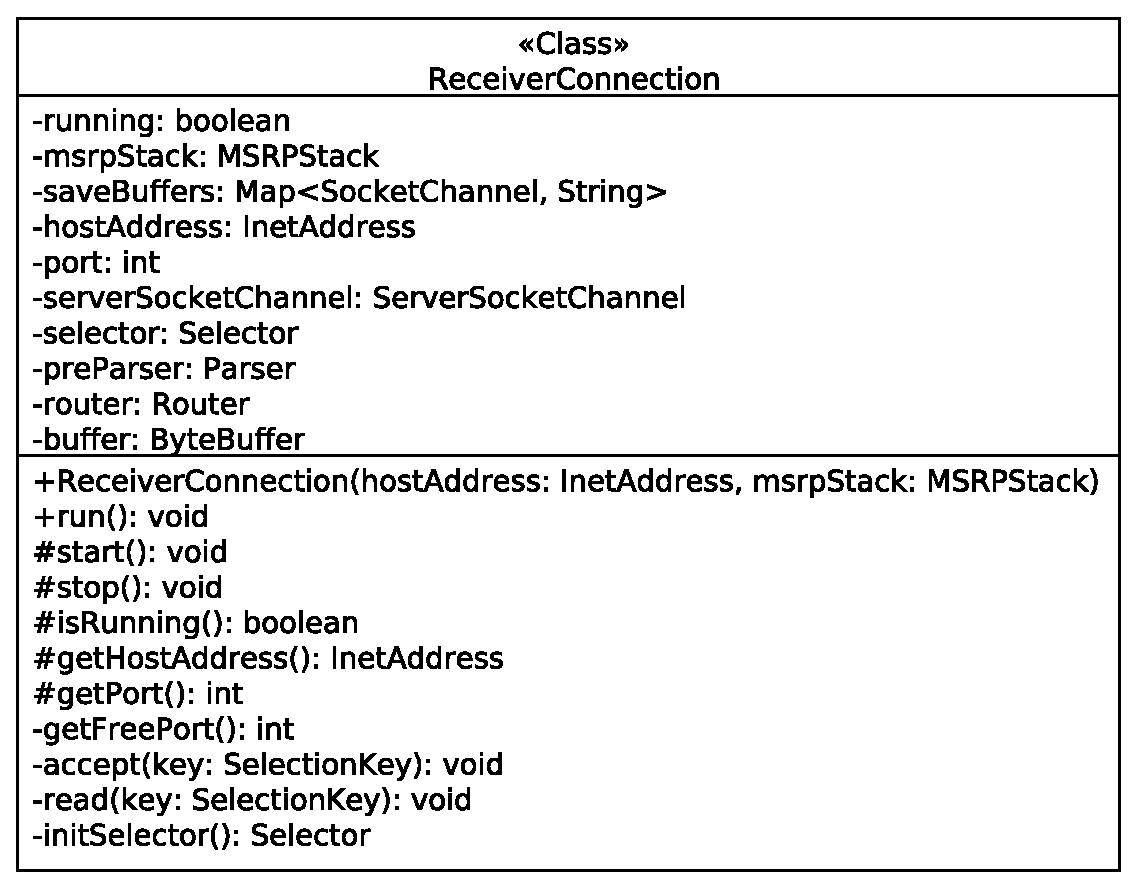
\includegraphics[width=0.43\textwidth]{img/class_diagrams/ReceiverConnection.eps}
  \end{center}
  \vspace{-15pt}
  \captionsetup{font=scriptsize}
  \caption{A ReceiverConnection osztálydiagramja}
   \label{fig:class_receiverconnection}
  \vspace{-10pt}
\end{wrapfigure}
A osztály felépítése \aref{fig:class_receiverconnection}.~ábrán látható. Privát változókban tárolja a kapcsolat állapotát (\code{running}), valamint referenciát a kapcsolatot tartalmazó \code{MSRPStack} objektumra. Tárolja a TCP kapcsolatok leírását (hoszt cím, port), azok menedzselését (\code{serverSocketChannel, selector}) végző objektumokat is. Szintén privát változóban tárolja a TCP kapcsolaton beérkező bájtfolyamból olvasott részadatok átmeneti tárolását végző objektumot (\code{saveBuffers}). Két belső osztályt tartalmaz: a \code{Parser}, illetve a \code{Router} osztályokat. A \code{Parser} osztály feladata, hogy a TCP kapcsolaton beérkező bájtfolyamból MSRP csomagokat állítson elő, amelyeknek a további feldolgozását a \code{Router} osztály végzi. A \code{Router} feladata, hogy az MSRP csomagokat a csomaghoz tartozó MSRP kapcsolathoz eljuttassa. A \code{saveBuffers} mapben tárolja a TCP socketből olvasott bájtfolyam végét, azokat az adatokat, amelyek az utolsónak rekonstruált MSRP csomaghoz már nem tartoznak, viszont egy, az adott TCP socket-ből való későbbi olvasás során a következő MSRP csomag részeként használatosak.

\subsubsection*{A SenderConnection osztály}
\label{sec:msrp_senderconnection}

\begin{wrapfigure}{r}{0.45\textwidth}
  \vspace{-15pt}
  \begin{center}
    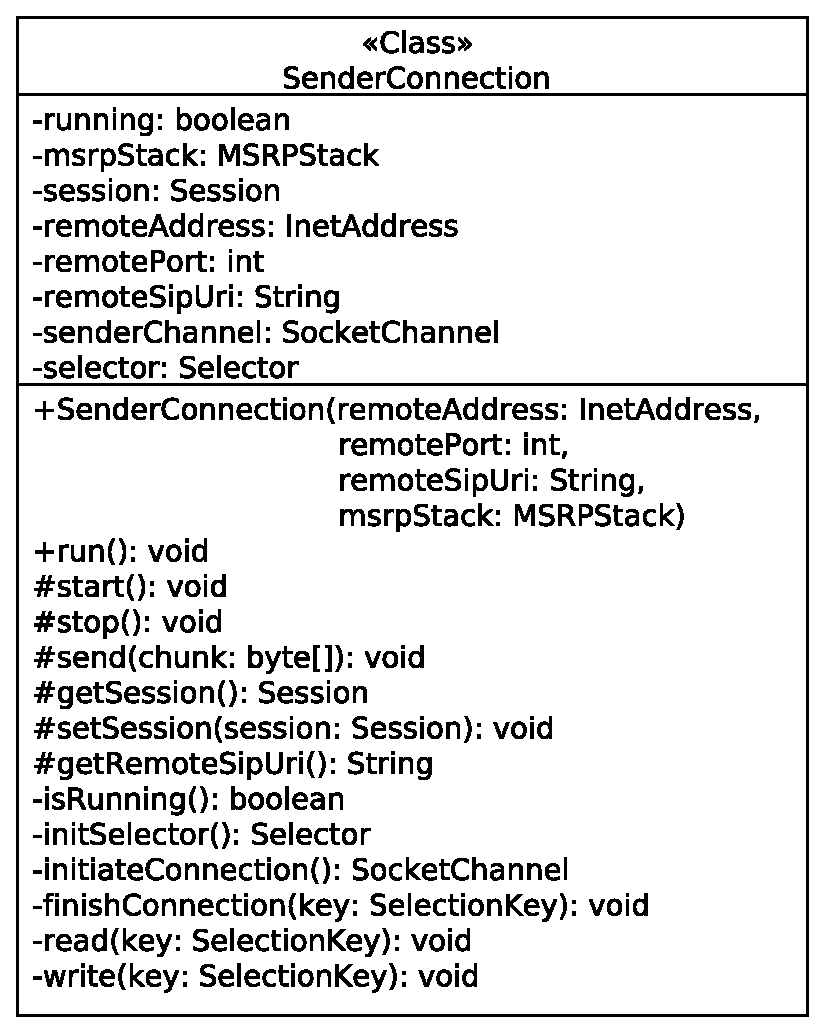
\includegraphics[width=0.43\textwidth]{img/class_diagrams/SenderConnection.eps}
  \end{center}
  \vspace{-15pt}
  \captionsetup{font=scriptsize}
  \caption{A SenderConnection osztálydiagramja}
   \label{fig:class_senderconnection}
  \vspace{-10pt}
\end{wrapfigure}
Az osztály az MSRP kapcsolaton (\code{session}), a \code{remoteSipUri} változóban tárolt SIP azonosítójú távoli félnek küldött MSRP csomagok továbbítását végzi. Minden különböző SIP URI-val rendelkező kommunikációs partnerhez tartozik egy \code{SenderConnection} példány, aminek egyedi azonosítására a \code{remoteSipUri} paraméter szolgál. A \code{ReceiverConnection} osztályhoz hasonlóan (\ref{sec:msrp_receiverconnection}.~pont) privát változókban tárolja a kapcsolat állapotát (\code{running}), referenciát az \code{MSRPStack} példányra, valamint a TCP kapcsolatot leíró, illetve vezérlő objektumokat. Az osztály által reprezentált TCP kapcsolaton a kapcsolat sikeres felépítése, valamint elindítása után adatot a \code{send} metódus meghívásával tudunk küldeni. A kapcsolat leállítását a \code{stop} metódus meghívásával idézhetjük elő.

\subsubsection*{A Session osztály}
\label{sec:msrp_session}

\begin{wrapfigure}{r}{0.45\textwidth}
  \vspace{-15pt}
  \begin{center}
    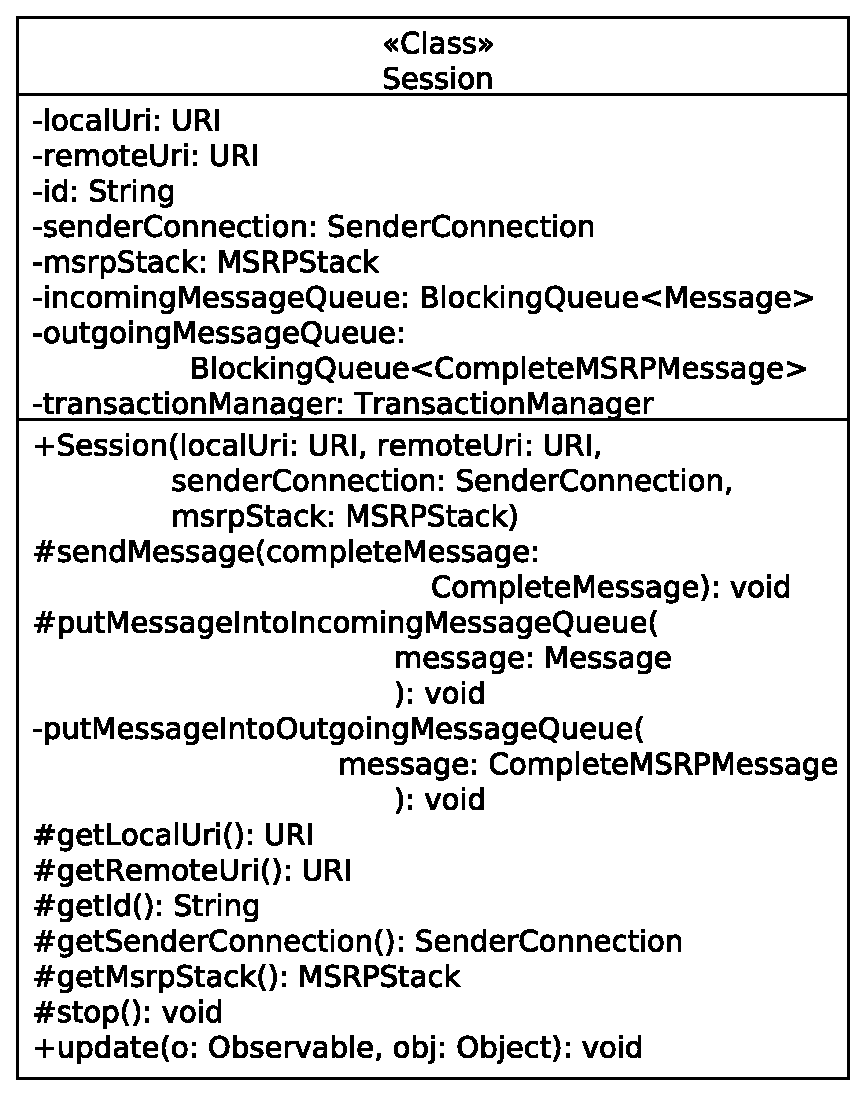
\includegraphics[width=0.43\textwidth]{img/class_diagrams/Session.eps}
  \end{center}
  \vspace{-15pt}
  \captionsetup{font=scriptsize}
  \caption{A Session osztálydiagramja}
   \label{fig:class_session}
  \vspace{-10pt}
\end{wrapfigure}
A \code{Session} osztály reprezentálja az MSRP kapcsolatot (\ref{fig:class_session}.~ábra). A \code{localURI} és a \code{remoteURI} változókban tárolódik a kapcsolatban résztvevő felek MSRP azonosítója. A \code{senderConnection} változóban az MSRP kapcsolathoz tartozó küldő TCP kapcsolatra referencia tárolódik. Az \code{incomingMessageQueue} sorba kerülnek az MSRP kapcsolathoz tartozó bejövő MSRP csomagok, míg az \code{outgoingMessageQueue} sorba az adott MSRP kapcsolaton küldendő MSRP üzenetek kerülnek. A sorokból a \code{session}-t kezelő \code{TransactionManager} osztálypéldány részeként az \code{IncomingMessageProcessor}, illetve az \code{OutgoingMessageProcessor} példányok dolgoznak. A \code{TransactionManager} osztály végzi az MSRP kérések tranzakcionált kezelését, azaz a kérések küldését, valamint a bejövő kérések nyugtázását. Az osztály, valamint a két processzor osztály leírása később, \aref{sec:msrp_transactionmanager}., \aref{sec:msrp_incomingprocessor}., valamint \aref{sec:msrp_outgoingprocessor}.~pontokban kerül kifejtésre. Az \code{id} változó az MSRP kapcsolat azonosítására szolgál, értéke a két URI konkatenációja. Utóbbi változó az \code{MSRPStack} osztályban lévő \code{activeSessions} mapben a kulcs attribútum. A \code{stop} metódus meghívásával az MSRP kapcsolat példányhoz kapcsolódó minden erőforrás felszabadításra kerül. 

\subsubsection*{A TransactionManager osztály}
\label{sec:msrp_transactionmanager}

\begin{wrapfigure}{r}{0.45\textwidth}
  \vspace{-25pt}
  \begin{center}
    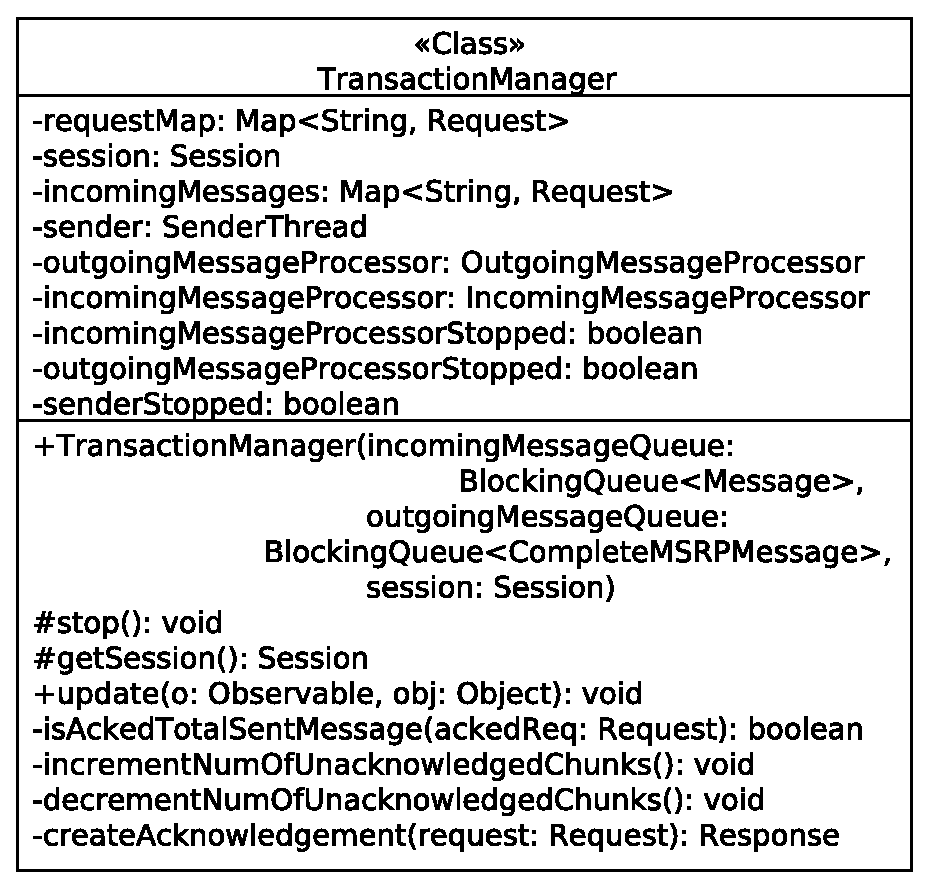
\includegraphics[width=0.43\textwidth]{img/class_diagrams/TransactionManager.eps}
  \end{center}
  \vspace{-15pt}
  \captionsetup{font=scriptsize}
  \caption{A TransactionManager osztálydiagramja}
   \label{fig:class_transactionmanager}
  \vspace{-10pt}
\end{wrapfigure}
A \code{TransactionManager} osztály (\ref{fig:class_transactionmanager}.~ábra) minden példánya egy-egy MSRP kapcsolat példányhoz (\code{session}) tartozik. Az MSRP kapcsolaton bejövő üzeneteket az \code{incomingMessageProcessor} példány továbbítja a \code{TransactionManager} példánynak. Hasonlóan, az MSRP kapcsolaton kiküldésre szánt üzenetet az \code{outgoingMessageProcessor} példány dolgozza fel, azaz teljes üzenetből MSRP kéréseket hoz létre, majd a kéréseket továbbítja a \code{TransactionManager} osztálynak, amely a tényleges küldéseket felügyeli. Az osztály a kiküldendő kéréseket egy mapben tárolja (\code{requestMap}), amelynek kulcsa az adott MSRP kérés tranzakció azonosítója. Amikor a kérésre nyugta érkezik (amit szintén megkap a \code{TransactionManager}), a nyugtához tartozó kérés törlődik az adott map-ből. A \code{TransactionManager} ezáltal tartja számon, hogy melyik kérésre nem érkezett még nyugta a távoli féltől. Az osztály másik feladata beérkező MSRP kérések nyugtázása. A beérkező kéréseket az \code{incomingMessages} mapben tárolódnak el. Miután az üzenethez tartozó utolsó MSRP kérés is megérkezett, a \code{TransactionManager} létrehoz egy MSRP eseményt, majd az \code{MSRPStack} példány \code{notifyListeners} metódusának meghívásával értesíti erről az aktuális MSRP kapcsolat eseményeire feliratkozott figyelőket.

\subsubsection*{Az OutgoingMessageProcessor osztály}
\label{sec:msrp_outgoingprocessor}
\begin{wrapfigure}{r}{0.45\textwidth}
  \vspace{-15pt}
  \begin{center}
    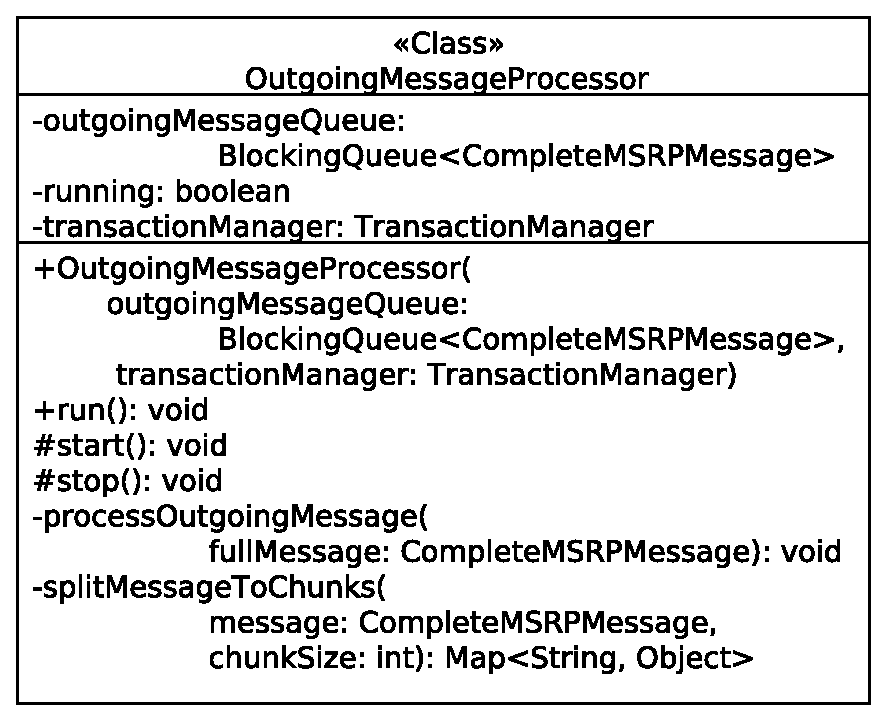
\includegraphics[width=0.43\textwidth]{img/class_diagrams/OutgoingMessageProcessor.eps}
  \end{center}
  \vspace{-15pt}
  \captionsetup{font=scriptsize}
  \caption{Az OutgoingMessageProcessor osztálydiagramja}
   \label{fig:class_outgoingprocessor}
  \vspace{-10pt}
\end{wrapfigure}

Az \code{OutgoingMessageProcessor} osztály osztálydiagramja \aref{fig:class_outgoingprocessor}.~ábrán látható. Feladata egyszerű, az MSRP kapcsolaton átvitelre szánt üzeneteket (\code{CompleteMSRPMessage} példányokat) kiolvassa a feldolgozási sorból (\code{outgoingMessageQueue}), azt meghatározott méretű darabokra tördeli (\code{splitMessageToChunks}), majd az egyes darabokból MSRP kéréseket generál, kitöltve a kérésekben szükséges paraméteket. A sikeres feldolgozás után a kérések listáját továbbítja a processzorhoz tartozó tranzakció menedzsernek (\code{transactionManager} változó). A \code{start} és a \code{stop} metódusok hívásával indítható, illetve leállítható a processzor működése. 

\subsubsection*{Az IncomingMessageProcessor osztály}
\label{sec:msrp_incomingprocessor}
\begin{wrapfigure}{r}{0.45\textwidth}
  \vspace{-15pt}
  \begin{center}
    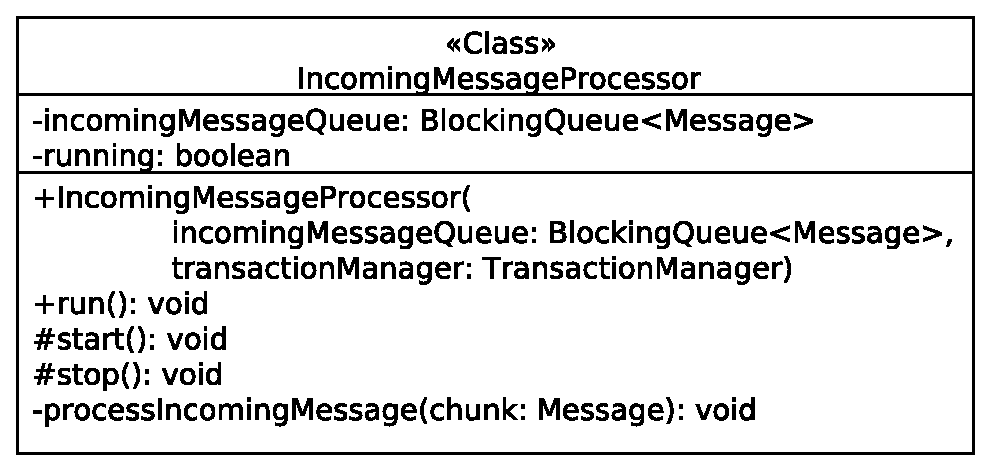
\includegraphics[width=0.43\textwidth]{img/class_diagrams/IncomingMessageProcessor.eps}
  \end{center}
  \vspace{-15pt}
  \captionsetup{font=scriptsize}
  \caption{Az OutgoingMessageProcessor osztálydiagramja}
   \label{fig:class_incomingprocessor}
  \vspace{-10pt}
\end{wrapfigure}
Az \code{IncomingMessageProcessor} osztály (\aref{fig:class_incomingprocessor}.~ábra) az MSRP kapcsolaton beérkező üzeneteket dolgozza fel. Az üzeneteket sorból olvassa (\code{incomingMessageQueue}), majd attól függően, hogy az MSRP üzenet kérés, vagy válasz, konvertálás után továbbítja azokat a processzort tartalmazó tranzakció menedzser példánynak. 

\subsubsection*{Az MSRPEvent osztály}
\label{sec:msrp_event}

\begin{wrapfigure}{r}{0.45\textwidth}
  \vspace{-15pt}
  \begin{center}
    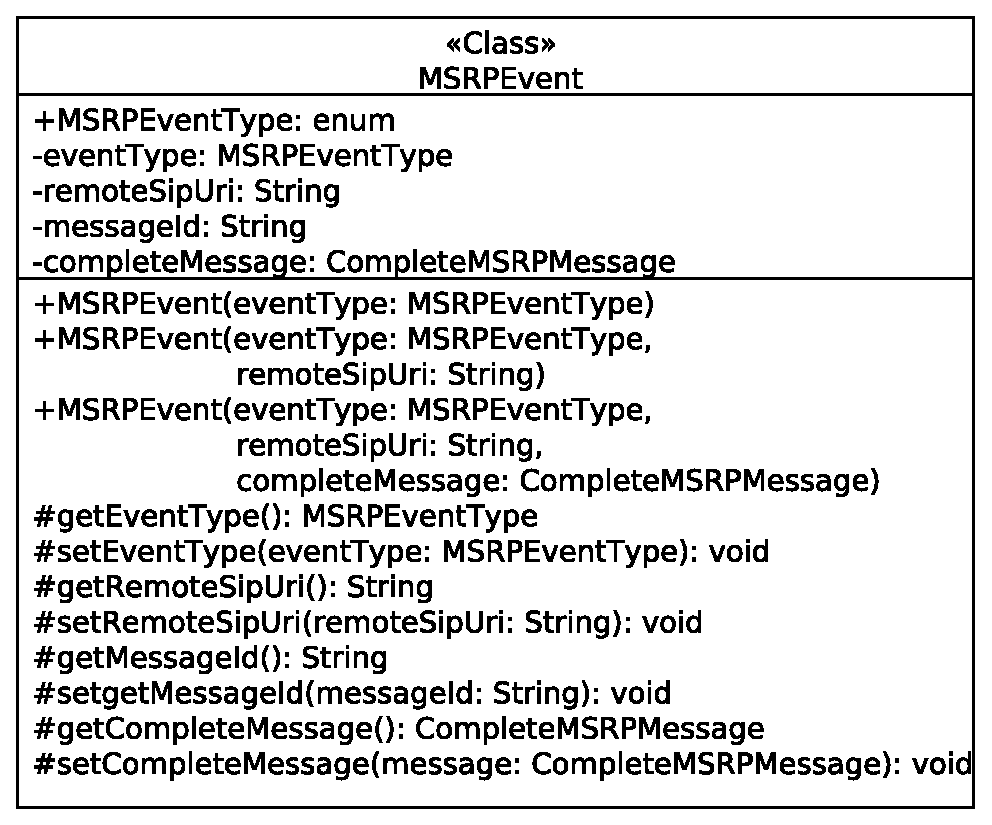
\includegraphics[width=0.43\textwidth]{img/class_diagrams/MSRPEvent.eps}
  \end{center}
  \vspace{-15pt}
  \captionsetup{font=scriptsize}
  \caption{Az MSRPEvent osztálydiagramja}
   \label{fig:class_event}
  \vspace{-10pt}
\end{wrapfigure}
Az \code{MSRPEvent} osztály reprezentálja az MSRP kapcsolatokban bekövetkezett eseményeket. Osztálydiagramja \aref{fig:class_event}.~ábrán tekinthető meg. A kapcsolatban bekövetkezett lehetséges események típusát a \code{MSRPEventType} felsorolás típus adja meg. Ilyen esemény típus lehet például egy MSRP kapcsolat sikeres létrehozása, vagy egy üzenet összes darabjának sikeres megérkezése, az MSRP kapcsolat megszakadása, stb. Privát változóban tárolja az MSRP kapcsolatban résztvevő távoli fél SIP azonosítóját (\code{remoteSipUri}). Opcionálisan megadható az üzenet azonosítója, amely üzenet átvitele során az esemény bekövetkezett. Az eseményben megadható maga, az MSRP kapcsolaton átvitelre került üzenet is (\code{completeMessage}), így az egyszerűen továbbítható azoknak az osztályoknak, akik feliratkoztak az eseményekre.

\subsubsection*{Az MSRPListener interfész}
\label{sec:msrp_listener}

\begin{wrapfigure}{r}{0.45\textwidth}
  \vspace{-15pt}
  \begin{center}
    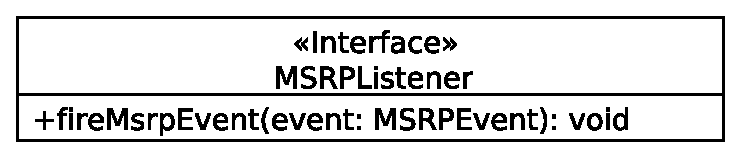
\includegraphics[width=0.43\textwidth]{img/class_diagrams/MSRPListener.eps}
  \end{center}
  \vspace{-15pt}
  \captionsetup{font=scriptsize}
  \caption{Az MSRPListener osztálydiagramja}
   \label{fig:class_listener}
  \vspace{-10pt}
\end{wrapfigure}
Az \code{MSRPListener} egy egyszerű interfész (\ref{fig:class_listener}.~ábra), amelynek \code{fireMSRPEvent} függvényének implementálásával az implementáló osztály az MSRP kapcsolatokban bekövetkezett eseményekről értesülhet. Ehhez annyit kell tenni, hogy az implementáló osztályt hozzá kell adni az \code{MSRPStack} osztály \code{msrpListeners} listájához (lásd.:\ref{sec:msrp_stack}.~pont)

\subsubsection*{Az MSRPUtil osztály}
\label{sec:msrp_util}

\begin{wrapfigure}{r}{0.45\textwidth}
  \vspace{-15pt}
  \begin{center}
    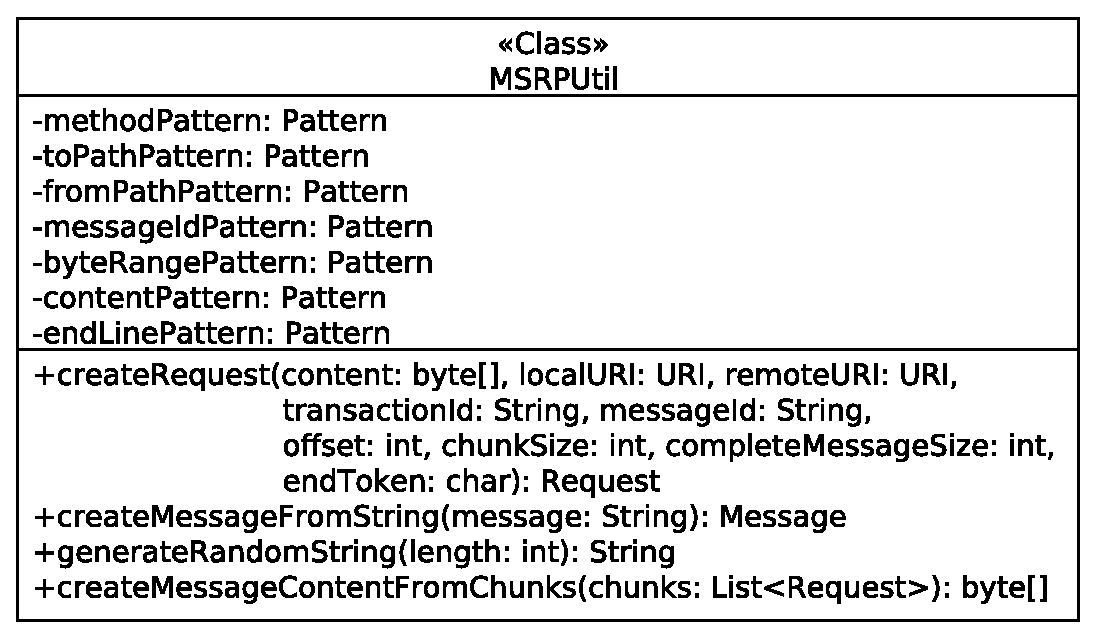
\includegraphics[width=0.43\textwidth]{img/class_diagrams/MSRPUtil.eps}
  \end{center}
  \vspace{-15pt}
  \captionsetup{font=scriptsize}
  \caption{Az MSRPUtil osztálydiagramja}
   \label{fig:class_util}
  \vspace{-10pt}
\end{wrapfigure}
Az \code{MSRPUtil} osztály (\ref{fig:class_util}.~ábra) négy statikus segédfüggvényt kínál az MSRP funkciókat megvalósító osztályoknak. A \code{createRequest} metódus segítségével a metódusnak paraméterben átadott adatokból egy MSRP kérést (\code{Request}) állít elő. A \code{createMessageFromString} metódus segítségével egy MSRP üzenet (\code{Message}) példányt hozhatunk létre. Az átadott String objektumban bizonyos mintákat keresünk, majd a talált minták alapján létrehozzuk az MSRP üzenetet. A \code{generateRandomString} egy adott hosszú véletlen karaktersorozatot ad vissza. A metódus a különböző azonosítók (üzenet azonosító, tranzakció azonosító, MSRP kapcsolat azonosító, stb.) generálására használatos. Végül a \code{createMessageContentFromChunks} metódussal a paraméterül átadott MSRP kérésekből visszaállítja az eredeti, MSRP kapcsolaton továbbított üzenetet.

\subsubsection*{A SessionDescription osztály}
\label{sec:msrp_sdp}

\begin{wrapfigure}{r}{0.45\textwidth}
  \vspace{-15pt}
  \begin{center}
    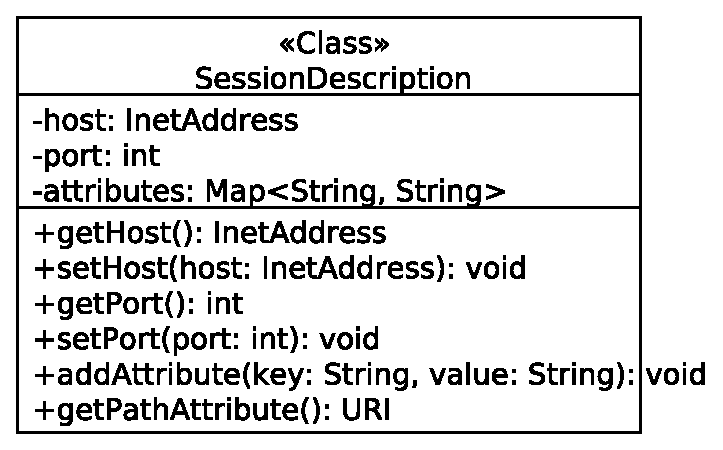
\includegraphics[width=0.43\textwidth]{img/class_diagrams/SessionDescription.eps}
  \end{center}
  \vspace{-15pt}
  \captionsetup{font=scriptsize}
  \caption{A SessionDescription osztálydiagramja}
   \label{fig:class_sdp}
  \vspace{-10pt}
\end{wrapfigure}

A \code{SessionDescription} osztály (\ref{fig:class_sdp}.~ábra) az MSRP kapcsolat SDP leíróját reprezentálja. Privát változóban tárolja az MSRP kapcsolat végpontjának IP címét (\code{host}), illetve portszámát (\code{port}). Mindkét paraméterhez lekérdező és beállító metódusok állnak rendelkezésre (code{getXY/setXY}). Privát map változóban tárolja a leíró attribútumait (\code{attributes}). Esetünkben, az MSRP kapcsolat SDP leíró esetén az attribútum map az elfogadott tartalom típusokat (accept-types), valamint a kapcsolatra jellemző URI-t (path) tartalmazza. Utóbbi értékét a \code{getPathAttribute} metódussal kérdezhetjük le.

\subsection{A kliens oldal megvalósítása}

A kliens alkalmazás egy grafikus alkalmazás, amely a felhasználói felület mellett tartalmazza a szerverrel való kommunikációért felelős osztályokat. A felület elemeinek megjelenítését, vezérlését, az események, adatok kezelését végző osztályok jelentős száma miatt ebben a részben részletesen csak a főbb funkciókat ellátó osztályokat mutatom be, összpontosítva csoportkezelésért felelős, illetve a szerverrel való kommunikációt végző osztályok bemutatására.

\subsubsection*{Az ICPController osztály}
\label{sec:client_icpcontroller}

\begin{wrapfigure}{r}{0.45\textwidth}
  \vspace{-15pt}
  \begin{center}
    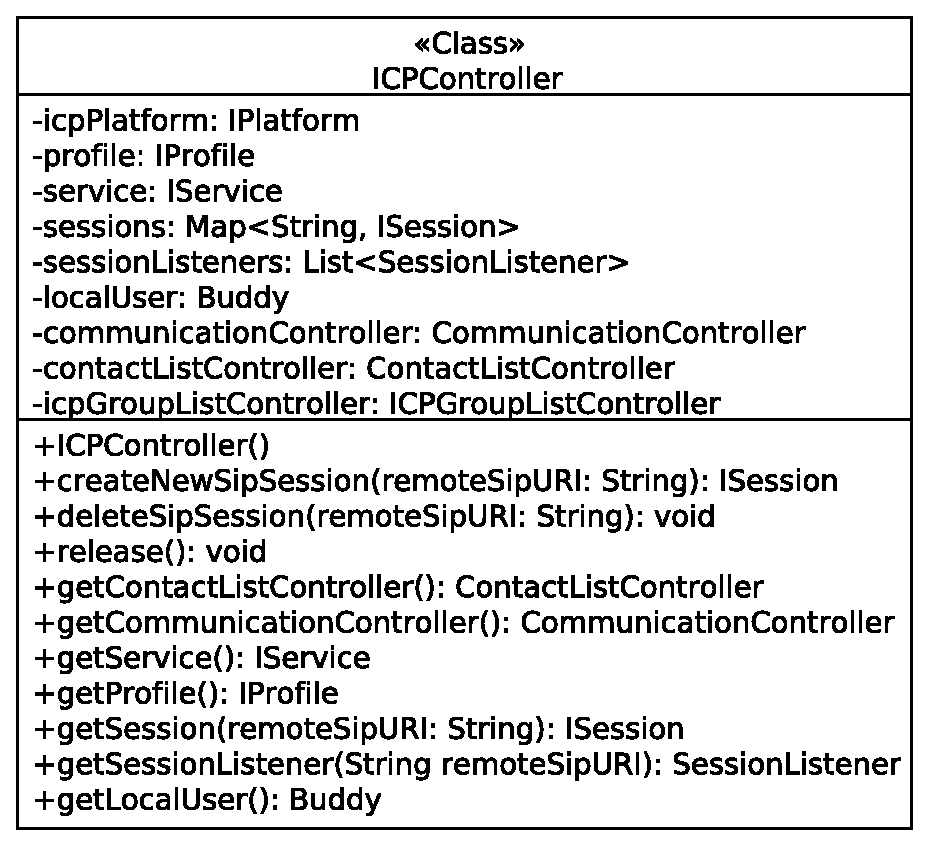
\includegraphics[width=0.43\textwidth]{img/class_diagrams/client/eps/ICPController.eps}
  \end{center}
  \vspace{-15pt}
  \captionsetup{font=scriptsize}
  \caption{Az ICPController osztálydiagramja}
   \label{fig:client_icpcontroller}
  \vspace{-10pt}
\end{wrapfigure}

Az \code{ICPController} osztály felépítése \aref{fig:client_icpcontroller}.~ábrán látható. Az osztály feladata az ICP nyújtotta funkciók elérése. Privát változóban tárolja a kommunikációs folyamatok vezérlését végző osztályt (\code{communicationController}), a csoportok menedzselését végző osztályokat (\code{contactListController}, \code{icpGroupListController}), valamint a kommunikációs felek között lévő aktív SIP kapcsolatokat. A SIP kapcsolatokban bekövetkezett eseményekről a \code{SessionListener} osztály értesíti az eseményekre feliratkozott osztályokat.

\begin{mycomment}
Kliens oldalon az alkalmazások számára az ICP előfeldolgozást végez a SIP üzeneteken~\cite{sds_dev_guide}. Amikor egy SIP üzenet megérkezik, az ICP egy eseményt generál, amely eseményeket a megfelelő listenerek tagfüggvényeinek implementálásával, valamint az eseményekre való feliratkozással lehet Java programból kezelni~\cite{sds_client_flow}. Például egy beérkező SIP MESSAGE üzenet hatására az ICP az \code{IServiceListener} interfész \code{processMessage} tagfüggvényét hívja meg. Másik példa, amikor egy SIP kapcsolat sikeresen felépül, az ICP a SIP kapcsolat eseményeire feliratkozott osztályokat az \code{ISessionListener} interfész \code{processSessionStarted} tagfüggvényével értesíti. Itt jegyezném meg, hogy a fentebb tárgyalt \code{ICPController} osztályban a \code{SessionListener} osztály éppen az \code{ISessionListener} interfész függvényeit implementálja, tehát a SIP kapcsolatokon bekövetkezett eseményekről értesíti az eseményekre feliratkozott osztályokat.
\end{mycomment}

\subsubsection*{A CommunicationController osztály}
\label{sec:client_communication_controller}

\begin{wrapfigure}{r}{0.45\textwidth}
  \vspace{-15pt}
  \begin{center}
    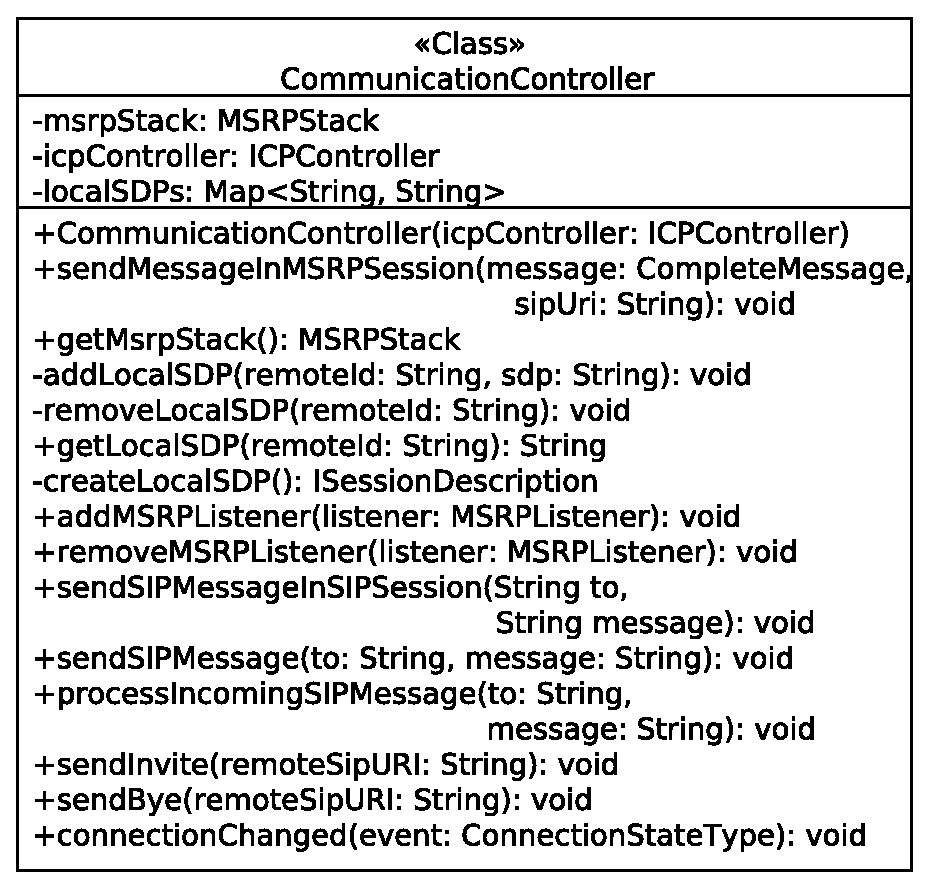
\includegraphics[width=0.43\textwidth]{img/class_diagrams/client/eps/CommunicationController.eps}
  \end{center}
  \vspace{-15pt}
  \captionsetup{font=scriptsize}
  \caption{A CommunicationController osztálydiagramja}
   \label{fig:class_client_communication_controller}
  \vspace{-10pt}
\end{wrapfigure}

A \code{CommunicationController} osztály (\ref{fig:class_client_communication_controller}.~ábra) végzi az alkalmazásban szükséges kommunikációs tevékenységeket. Nyílvános metódusokkal támogatja a kommunikációs folyamatokat. A \code{sendInvite} metódus meghívásával egy új MSRP kapcsolat építhető fel egy távoli féllel, míg egy létező MSRP kapcsolaton üzenetet küldeni a \code{sendMessageInMSRPSession} metódus meghívásával lehet. MSRP kapcsolatot bontani a \code{sendBye} függvény meghívásával lehet. SIP MESSAGE üzenetet a \code{sendSIPMessage} metódussal, míg egy felépített SIP kapcsolaton a \code{sendSIPMessageInSIPSession} metódus megfelelő meghívásával lehet. Az osztály segítségével lehetőség nyílik fel/leirakozni az MSRP kapcsolatok eseményeire. További feladatként a beérkező SIP üzenetek feldolgozását is a \code{CommunicationController} osztály végzi. A létrehozott SIP kapcsolatokon bekövetkezett eseményeketről értesül, és az események hatására végrehajtja a szükséges akciókat (például egy SIP kapcsolat sikeres elindulását jelző esemény hatására létrehozza az MSRP kapcsolatot).

\subsubsection*{A ContactListController osztály}
\label{sec:client_contactlistcontroller}

\begin{wrapfigure}{r}{0.45\textwidth}
  \vspace{-15pt}
  \begin{center}
    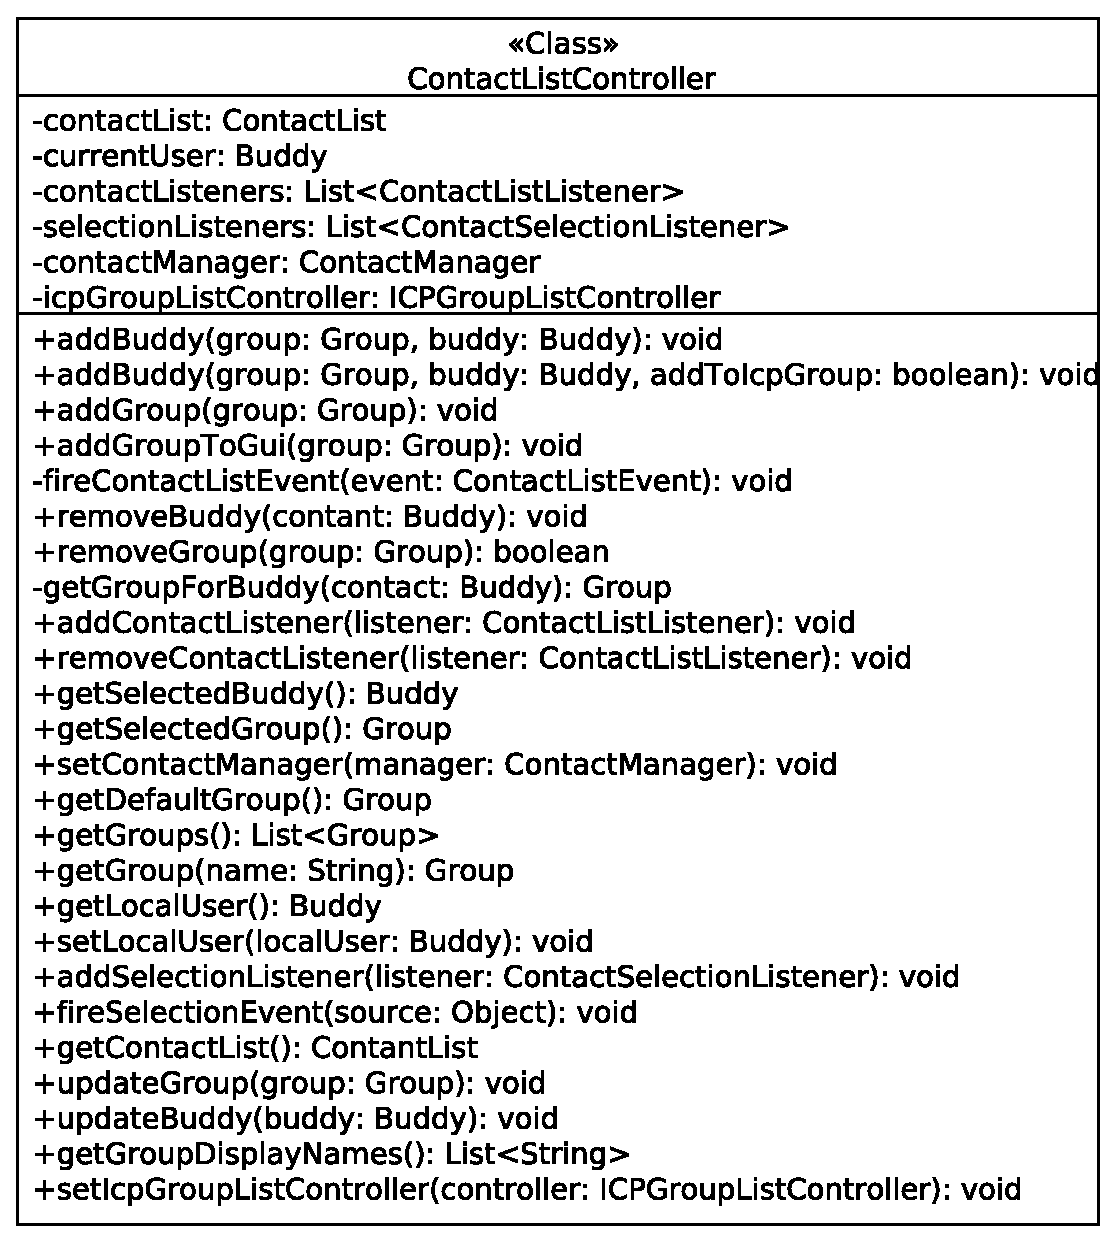
\includegraphics[width=0.43\textwidth]{img/class_diagrams/client/eps/ContactListController.eps}
  \end{center}
  \vspace{-15pt}
  \captionsetup{font=scriptsize}
  \caption{A ContactListController osztálydiagramja}
   \label{fig:class_client_contactlistcontroller}
  \vspace{-10pt}
\end{wrapfigure}

A \code{ContactListController} osztály (\ref{fig:class_client_contactlistcontroller}.~ábra) feladata összefogni, illetve egységesen kezelni a PGM szerveren, a lokális tárban, valamint a grafikus felületen megjelenő kapcsolati listákat, illetve a csoportokban bekövetkezett változásokról értesíteni az egyes, csoportokkal kapcsolatos funkciókat megvalósító osztályokat (pl. a csoportokat megjelenítő grafikus felületet). Az osztályban megtalálható egy, a csoportokat tartalmazó lista (\code{contactList}), amely a helyi csoportlisták tárolását, valamint menedzselését végzi, mint pl. új csoport létrehozása, vagy egy kiválasztott csoporthoz új tag felvétele. Tartalmaz egy kontroller osztályt (\code{icpGroupListController}), amely az SDS-ben megtalálható PGM szerveren végrehajtandó funkciókat látja el, úgymint a lokális csoportlista és a PGM szerveren tárolt csoportlista egymással való szinkronizációja. A \code{ContactListController} osztály tagfüggvényei főleg a csoportok menedzselését végzik, mint egy csoport létrehozása vagy törlése, új csoporttagok felvétele, a tagok módosítása, vagy törlése, stb. A grafikus felületen kiválasztott csoport, vagy csoporttag adatai lekérdezhetőek (\code{getSelectedBuddy/Group}).

\medskip

A kliens alkalmazást megvalósító osztályok közül a multimédia üzenetek táblázatos formában való megjelenítését a \code{MessageBoxDialog} osztály végzi, amely külön listában tartalmazza az elküldött és a bejövő multimédia üzeneteket. Egy kiválaszott üzenet részleteinek megjelenítését, az üzenet tartalmának típusától függően a \code{MessageDetails} osztályból leszármazott osztályok végzik. Hangüzenet megjelenítését az \code{AudioMessageDetails}, képüzenet megjelenítését az \code{ImageMessageDetails}, míg videóüzenet részleteinek megjelenítését a \code{VideoMessageDetails} osztály végzi. Üzenetet törölni szintén a \code{MessageBoxDialog} osztály segítségével lehet. 

\medskip

Egy multimédia üzenet adatainak kliens oldali perzisztens (merevlemezen történő) tárolása az értesítő MESSAGE üzenetben küldött XML-hez hasonló felépítésű fájlban történik. Az üzenethez tartozó multimédia tartalom -- amennyiben a tartalom kliens oldalon elérhető -- az XML fájl mellett található meg. A kliens oldali XML-ek Java objektumokká konvertálását, a multimédia üzenetek feldolgozását, betöltését, fájlba írását az \code{XMLUtils}, valamint a \code{MessageUtils} osztályok végzik.

\medskip

Egy új multimédia üzenet létrehozását, illetve küldését a \code{SendMessageDialog} osztály végzi. A tartalom létrehozását egyéb osztályok felhasználásával végzi. A Java nyelvben megtalálható Java Media Framework (JMF) keretrendszer \cite{jmf} fejlesztői API-val támogatást ad a számítógépben megtalálható hang, illetve videó eszközök kezelésére. A fejlesztés során a multimédia tartalom készítéséhez a JMF nyújtotta fejlesztői API-t használtam. A multimédia tartalom létrehozásához szükséges funkciókat a \code{CaptureDialog} osztály nyújtja. A \code{CaptureDialog} osztályon belül több segédosztály is megtalálható. Hang felvétel készítését az \code{AudioRecorder} osztály végzi, a hangfelvétel wav-ból mp3 formátumba történő konverziójának feladatát az \code{AudioConverter} osztály oldja meg. Kép, illetve videó felvétel a \code{VideoRecorder} osztály felhasználásával készíthető. A \code{SendMessageDialog} osztály az elkészült multimédia üzenet küldése során felhasználja a \code{CommunicationController} osztály nyújtotta funkciókat.


\subsection{A szerver oldal megvalósítása}

A most következő részben bemutatom a szerver oldali szolgáltatás megvalósításának fontosabb osztályait, ábrán prezentálva az osztályok felépítését. Természetes itt is csak a fontosabb osztályok tárgyalása következik, a teljes szerver oldali alkalmazás részletezése túlmutat a dolgozat keretein.

\subsubsection*{A MessagingService osztály}
\label{sec:server_messagingservice}

\begin{wrapfigure}{r}{0.45\textwidth}
  \vspace{-15pt}
  \begin{center}
    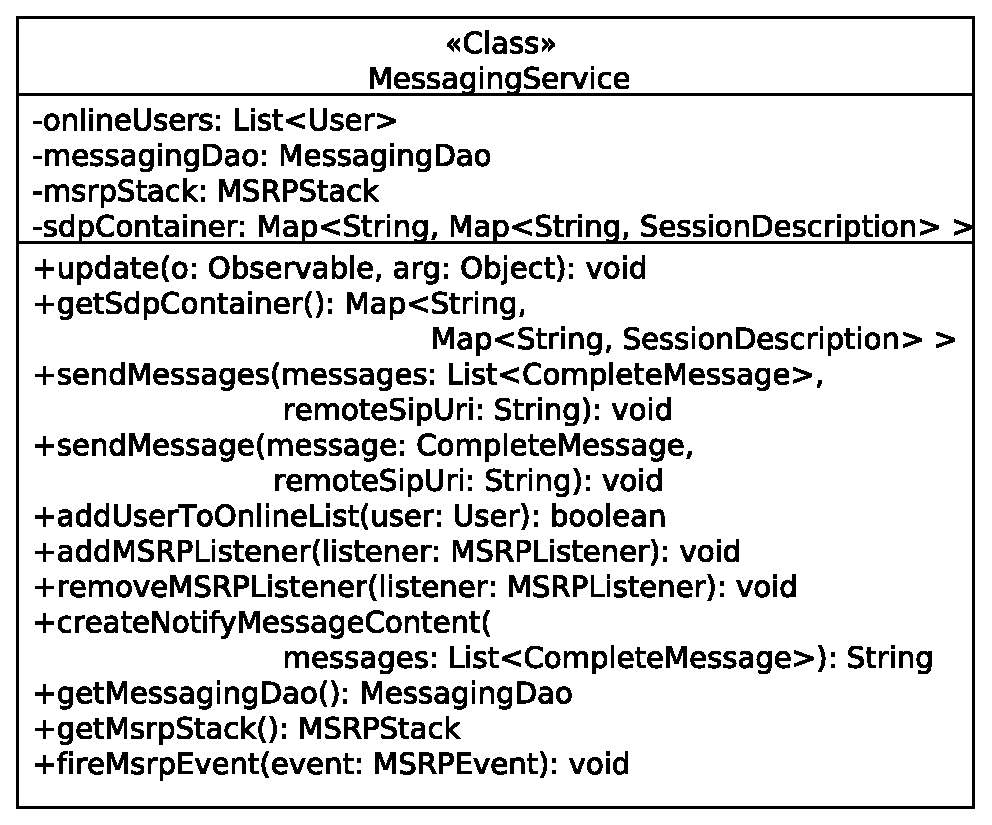
\includegraphics[width=0.43\textwidth]{img/class_diagrams/server/eps/MessagingService.eps}
  \end{center}
  \vspace{-15pt}
  \captionsetup{font=scriptsize}
  \caption{A MessagingService osztálydiagramja}
   \label{fig:class_server_messagingservice}
  \vspace{-10pt}
\end{wrapfigure}

A \code{MessagingService} osztály felépítése \aref{fig:class_server_messagingservice}.~ábrán látható. Ez az osztály az üzenetküldő szolgáltatásban egyrészt az MSRP protokoll stack funkcióinak elérését teszi lehetővé, úgymint egy új MSRP kapcsolat felépítése, vagy egy felépített MSRP kapcsolaton adott multimédia üzenet tartalmának átvitele. A \code{MessagingService} osztály listában tárolja az IMS hálózaton regisztrált, elérhető felhasználókat (\code{onlineUsers}). Szintén privát változóban tárolja az MSRP protokollt megvalósító, \aref{sec:msrp_implementacio}.~fejezetben tárgyalt \code{MSRPStack} osztály példányát. Az \code{sdpContainer} mapben tárolja az kliens-szerver között aktív MSRP kapcsolatok SDP leíróit. Mivel egy kliens és a szerver között egyszerre csak egy aktív MSRP kapcsolat lehet, ezért a map a felhasználó SIP URI-ját használja kulcs attribútumként. Az SDP-k eltárolása azért szükséges, mivel egy adott klienssel a tényleges MSRP kapcsolat csak a klienssel történő INVITE~--~200~OK~--~ACK üzenetváltás sikeres befejeződése után jön létre. Az MSRP kapcsolat létrehozásához viszont szükség van mint az INVITE-ban érkező kliens SDP leírójára, mint a szerver oldalon generált SDP leíróra.

A \code{MessagingService} osztály további változóban tárolja az adatbázis eléréséhez szükséges funkciókat biztosító \code{MessagingDao} osztály egy példányát. 

A \code{MessagingService} osztály implementálja az \code{MSRPListener} interfészt, valamint feliratkozik az MSRP kapcsolatokon bekövetkezett eseményekre, ezáltal az egyes események határása végre tudja hajtani a szükséges lépéseket (Például egy kliens felől érkező multimédia üzenet tartalmának sikeres megérkezése után eltárolja az adatbázisban).

\subsubsection*{A MessagingSipServlet osztály}
\label{sec:server_messagingsipservlet}

\begin{wrapfigure}{r}{0.45\textwidth}
  \vspace{-15pt}
  \begin{center}
    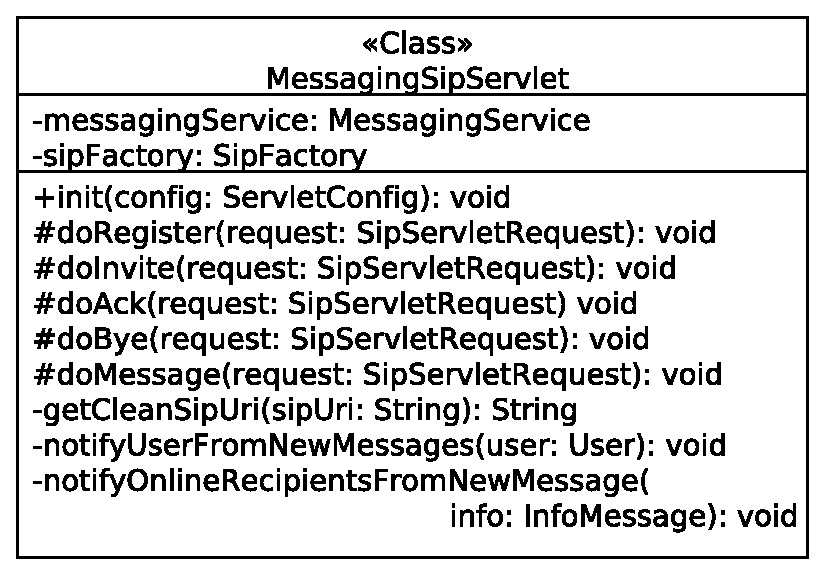
\includegraphics[width=0.43\textwidth]{img/class_diagrams/server/eps/MessagingSipServlet.eps}
  \end{center}
  \vspace{-15pt}
  \captionsetup{font=scriptsize}
  \caption{A MessagingSipServlet osztálydiagramja}
   \label{fig:class_server_messagingsipservlet}
  \vspace{-10pt}
\end{wrapfigure}

A \code{MessagingSipServlet} osztály (\ref{fig:class_server_messagingsipservlet}.~ábra) a Java API részét képező \code{SipServlet} osztály leszármazottja. Az osztály feladata a kliensektől érkező, különböző típusú SIP üzenetek feldolgozása, a megfelelő lépések végrehajtása, illetve a üzenetekre a szükséges válaszüzenetek küldése. Privát változóban tárolja az üzenetküldő szolgáltatás magját képező \code{MessagingService} osztály egy példányát, amely osztály funkcióit használva kiszolgálja a kliensek különféle igényeit, mint pl. egy felépített MSRP kapcsolaton egy multimédia üzenet tartalmának letöltése, vagy akár egy új üzenet vételekor az elérhető címzetteknek értesítő üzenet küldése.

\subsubsection*{A MessagingDao osztály}
\label{sec:server_messagingdao}

\begin{wrapfigure}{r}{0.45\textwidth}
  \vspace{-15pt}
  \begin{center}
    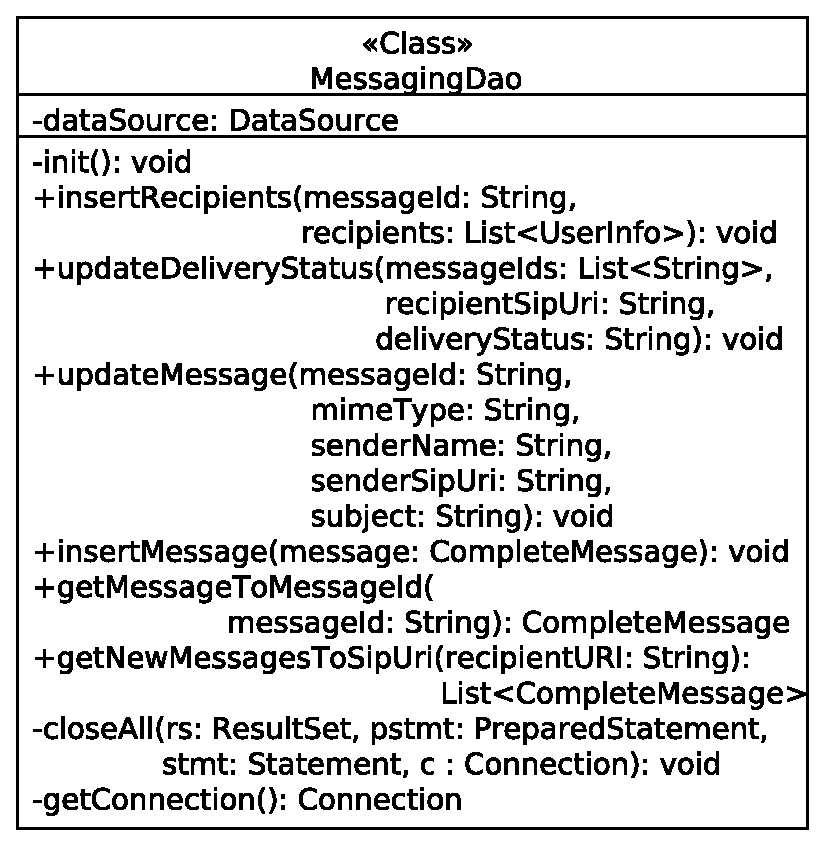
\includegraphics[width=0.43\textwidth]{img/class_diagrams/server/eps/MessagingDao.eps}
  \end{center}
  \vspace{-15pt}
  \captionsetup{font=scriptsize}
  \caption{A MessagingDao osztálydiagramja}
   \label{fig:class_server_messagingdao}
  \vspace{-10pt}
\end{wrapfigure}

A \code{MessagingDao} osztály a különféle adatbázis műveletek végrehajtását végzi. Osztálydiagramja \aref{fig:class_server_messagingdao}.~ábrán tekinthető meg. A szolgáltatásnak nyílvános metódusokat nyújt az adatbázissal való kommunikációra. Segítségével egy multimédia üzenetet, annak címzettjeit adatbázisba beszúrhatjuk (\code{insertMessage}, \code{insertRecipients}), egy üzenet adatait frissíthetjük (\code{updateMessage}), vagy egy adott üzenethez tartozó címzett bejegyzés kézbesítési státuszát módosíthatjuk (\code{updateDeliveryStatus}) egy megadott állapotra. Az osztály felhasználásával a következő adatbázis lekérdező műveleteket hajthatunk végre: lekérdezhetjünk egy adott üzenet azonosítóval rendelkező multimédia üzenet adatait (\code{getMessagesToMessageId}), vagy megkaphatjuk egy adott felhasználó új multimédia üzeneteit (\code{getNewMessagesToSipUri}). A \code{closeAll} privát metódus a paraméterében átadott objektumok által foglalt erőforrásokat szabadítja fel.

\medskip

A fentebb tárgyalt osztályok a következő további osztályokat használják. A \code{CompleteMessage} osztály adattárolási funkciót lát el, paraméterben tárolja a multimédia üzenet tartalmát, annak típusát, az üzenet azonosítóját, a feladó nevét és SIP URI-ját, valamint a multimédia üzenet tárgyát és a küldési időpontot.

\medskip

A \code{User} osztály az elérhető, azaz regisztrált felhasználok SIP URI-ját tartalmazza, továbbá egy időzítőt, amely a felhasználótól érkező SIP REGISTER üzenet lejárati idejéről számol visszafelé. Az adott felhasználótól érkező minden REGISTER üzenet újraindítja az időzítőt. Amikor az időzítő lejár, a \code{MessagingService} osztály az adott felhasználót törli az elérhető felhasználók listájából (\code{onlineUsers}).

\medskip

Az XML-ek feldolgozását, az XML--objektum konverziót szerver oldalon -- hasonlóan a klienshez -- egy \code{XMLUtils} nevű osztály végzi.